\documentclass[border=12pt]{standalone}
\def\pgfsysdriver{pgfsys-dvisvgm.def}
\usepackage[dvisvgm]{xcolor}
\usepackage{xeCJK}
\setCJKmainfont{HaranoAjiGothic-Regular.otf}[BoldFont=HaranoAjiGothic-Bold.otf]
\setCJKsansfont{HaranoAjiGothic-Regular.otf}[BoldFont=HaranoAjiGothic-Bold.otf]
\usepackage{amsmath,amssymb,tikz,lmodern}
\usetikzlibrary{arrows.meta,positioning,calc,fit,backgrounds}
\renewcommand{\familydefault}{\sfdefault}
\definecolor{ink}{HTML}{25322F}
\definecolor{green}{HTML}{246657}
\definecolor{tint}{HTML}{EEF4F0}
\definecolor{soft}{HTML}{C6D2CC}
\definecolor{muted}{HTML}{52615B}
\newif\ifJapanese
\newcommand{\Tx}[2]{\ifJapanese #1\else #2\fi}
\newcommand{\Eff}{\overline{\operatorname{Eff}}}
\newcommand{\heading}[3]{{\color{green}\bfseries #1\quad\Tx{#2}{#3}}\\[5pt]}
% A white rectangle makes the complete citation label clickable, including spaces.
\newcommand{\refurl}[2]{\special{dvisvgm:raw <a xlink:href="#1" target="_blank" rel="noopener noreferrer">}{\setlength{\fboxsep}{0pt}\colorbox{white}{\color{green}\underline{\strut #2}}}\special{dvisvgm:raw </a>}}
\tikzset{
 card/.style={draw=soft,fill=white,rounded corners=2pt,align=left,text=ink,font=\fontsize{10.5}{14}\selectfont,inner xsep=12pt,inner ysep=10pt,text width=16cm},
 half/.style={card,text width=7.1cm,minimum height=2.05cm},
 result/.style={draw=green,fill=tint,line width=.9pt},
 reason/.style={align=left,text=muted,font=\fontsize{9}{12}\selectfont,inner sep=0pt,text width=14.3cm},
 branchreason/.style={reason,text width=6.4cm},
 edge/.style={-{Stealth[length=2.4mm]},draw=green,line width=1pt},
 wire/.style={draw=green,line width=1pt},
}
% Keep the arrow in a dedicated left gutter; explanations never cover it.
\newcommand{\flow}[3]{
 \coordinate (#2-from) at ($(#1.south)+(-7.7,0)$);
 \coordinate (#2-to) at ($(#2.north)+(-7.7,0)$);
 \draw[edge] (#2-from)--(#2-to);
 \node[reason,anchor=west] (#2-reason) at ($(#2-from)!.5!(#2-to)+(.55,0)$) {#3};
}

\newcommand{\RA}[1]{\refurl{\sourceRA}{#1}}
\newcommand{\OI}[1]{\refurl{\sourceOI}{#1}}
\newcommand{\FF}[1]{\refurl{\sourceFF}{#1}}
\newcommand{\FFcor}[1]{\refurl{\sourceFFcor}{#1}}
\newcommand{\BBT}[1]{\refurl{\sourceBBT}{#1}}
\newcommand{\FG}[1]{\refurl{\sourceFG}{#1}}
\newcommand{\CP}[1]{\refurl{\sourceCP}{#1}}
\newcommand{\BDPP}[1]{\refurl{\sourceBDPP}{#1}}
\newcommand{\pe}{\mathrel{\geq_{\mathrm{pe}}}}
\newcommand{\rowflow}[3]{
 \coordinate (#2-a) at ($(#1.south)+(-3.45,0)$);
 \coordinate (#2-b) at ($(#2.north)+(-3.45,0)$);
 \draw[edge] (#2-a)--(#2-b);
 \node[branchreason,anchor=west] at ($(#2-a)!.5!(#2-b)+(.45,0)$) {#3};
}

\newcommand{\sourceRA}{https://github.com/openai/math/blob/fd4aeeb2ee4fc729c18d98444fed42fd0529eeeb/preprints/The-reverse-logarithmic-Kodaira-inequality-and-additivity-September-26-2026/paper.pdf}
\newcommand{\sourceOI}{https://github.com/openai/math/blob/fd4aeeb2ee4fc729c18d98444fed42fd0529eeeb/preprints/Orbifold-and-logarithmic-Iitaka-subadditivity-September-26-2026/paper.pdf}
\newcommand{\sourceFF}{https://www.math.kyoto-u.ac.jp/~fujino/vmhs-sp108.pdf}
\newcommand{\sourceFFcor}{https://www.math.kyoto-u.ac.jp/~fujino/fujino-fujisawa-memo2.pdf}
\newcommand{\sourceBBT}{https://arxiv.org/pdf/1811.12230v3}
\newcommand{\sourceFG}{https://www.numdam.org/item/10.5802/aif.2894.pdf}
\newcommand{\sourceCP}{https://arxiv.org/pdf/1508.02456v4}
\newcommand{\sourceBDPP}{https://arxiv.org/pdf/math/0405285v1}
\Japanesefalse
\begin{document}
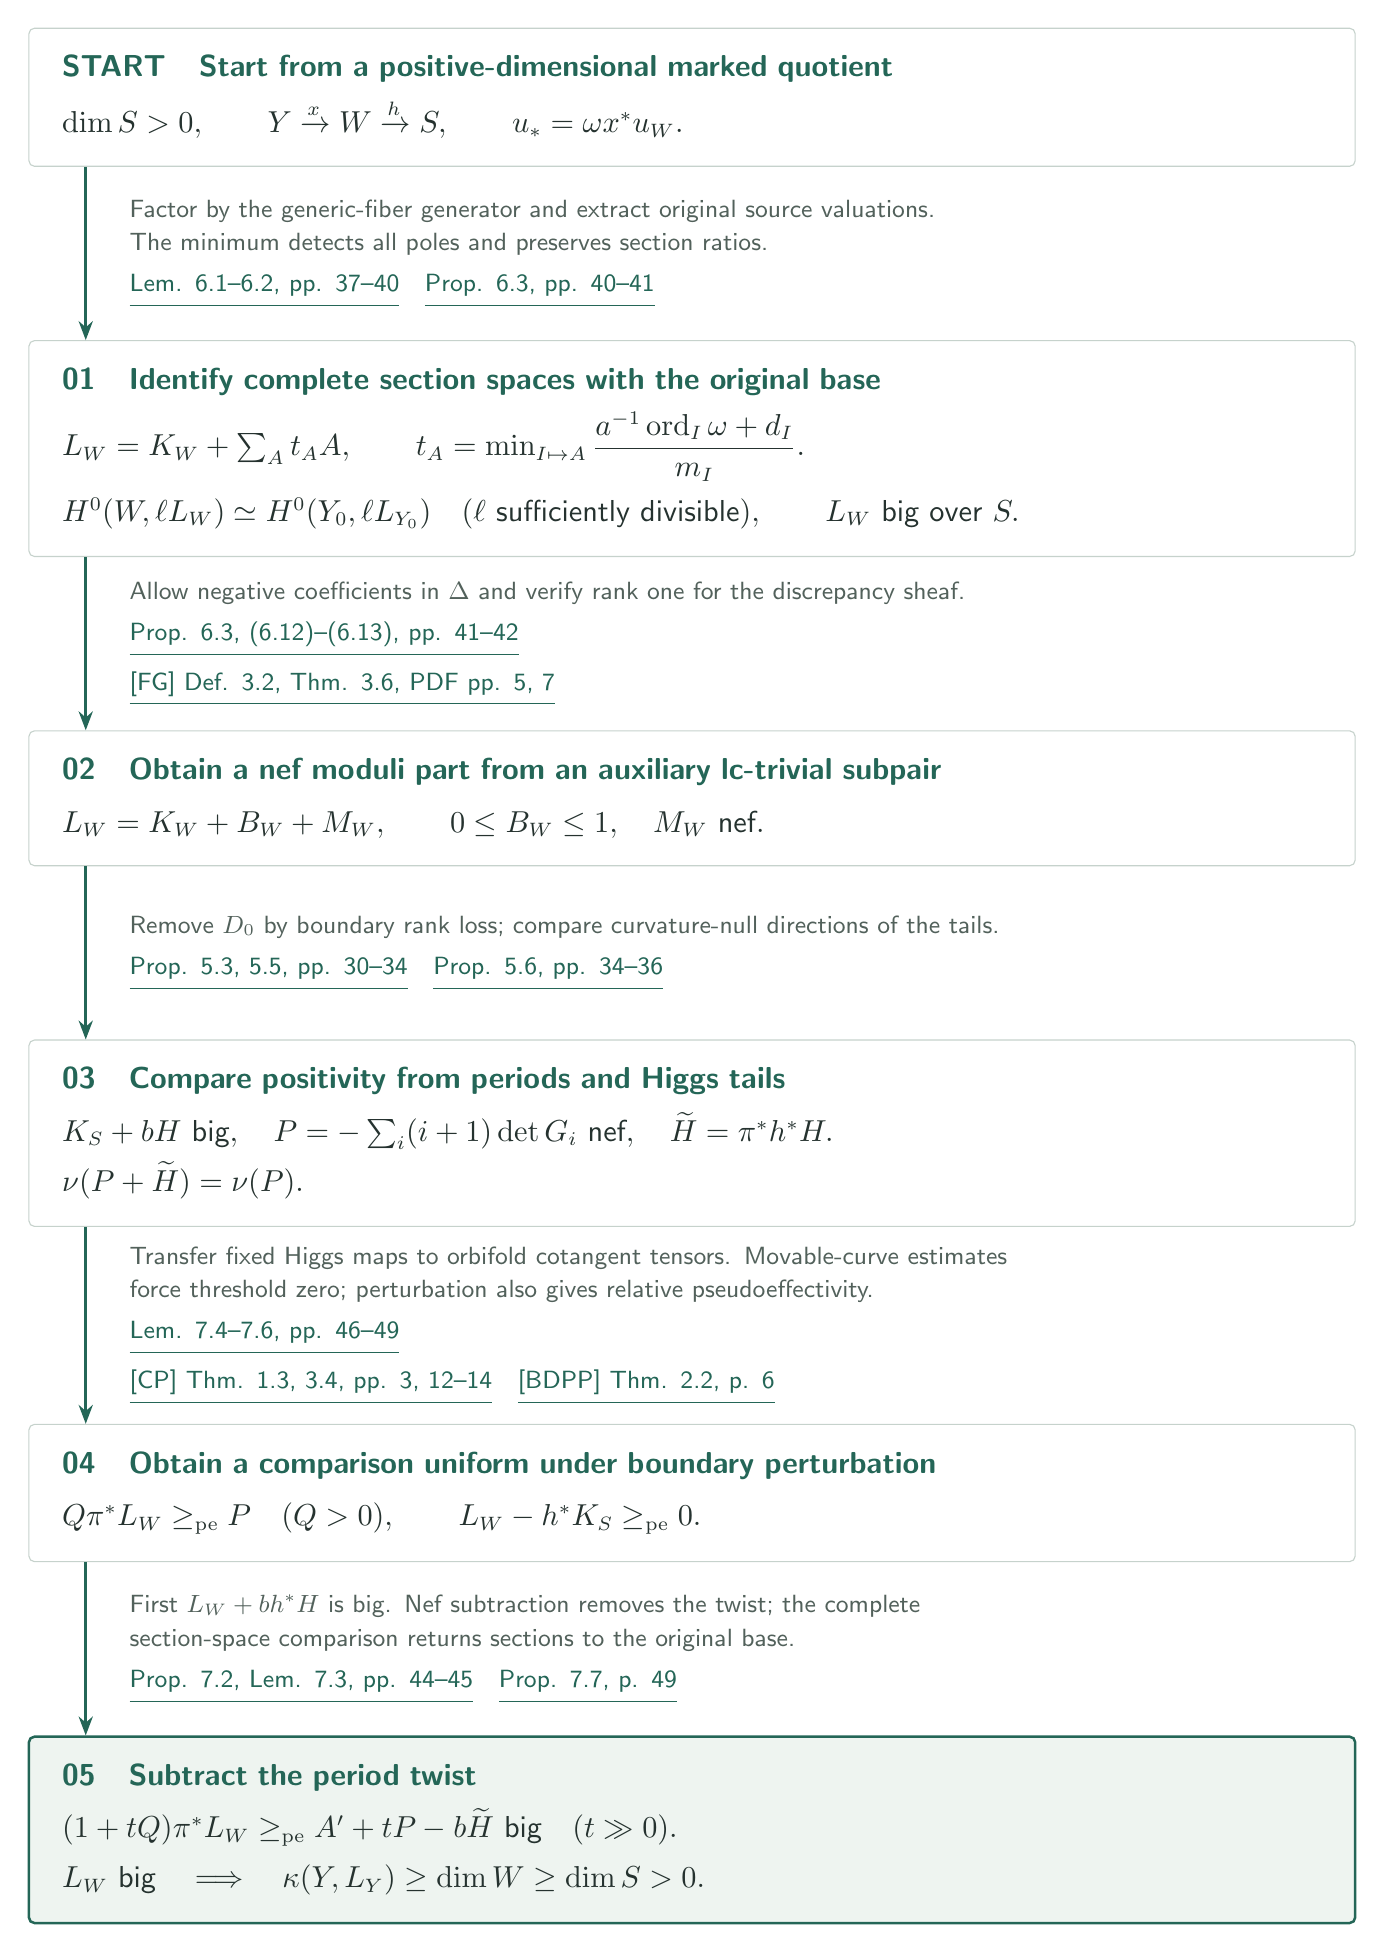
\begin{tikzpicture}
\node[card] (start) {\heading{START}{正次元のmarked quotientから出発する}{Start from a positive-dimensional marked quotient}
$\dim S>0,\qquad Y\xrightarrow{x}W\xrightarrow{h}S,\qquad u_*=\omega x^*u_W.$};
\node[card,below=2.2cm of start] (lattice) {\heading{01}{元の底と完全切断空間を一致させる}{Identify complete section spaces with the original base}
$L_W=K_W+\sum_A t_AA,\qquad t_A=\min_{I\mapsto A}\dfrac{a^{-1}\operatorname{ord}_I\omega+d_I}{m_I}.$\\[5pt]
$H^0(W,\ell L_W)\simeq H^0(Y_0,\ell L_{Y_0})\quad(\ell\ \Tx{\text{十分割り切れる}}{\text{sufficiently divisible}}),\qquad L_W\ \text{big over }S.$};
\flow{start}{lattice}{\Tx{generic fiberの生成元で分解し、元のsourceのvaluationを抽出する。\\最小値の条件が全ての極を検出し、切断比を保つ。}{Factor by the generic-fiber generator and extract original source valuations.\\The minimum detects all poles and preserves section ratios.}\\[3pt]\RA{Lem. 6.1--6.2, pp. 37--40}\quad\RA{Prop. 6.3, pp. 40--41}}
\node[card,below=2.2cm of lattice] (nef) {\heading{02}{lc-trivialな補助subpairからnef部分を得る}{Obtain a nef moduli part from an auxiliary lc-trivial subpair}
$L_W=K_W+B_W+M_W,\qquad 0\leq B_W\leq1,\quad M_W\ \text{nef}.$};
\flow{lattice}{nef}{\Tx{負の係数を許す $\Delta$ で、discrepancy sheafの階数1を検証する。}{Allow negative coefficients in $\Delta$ and verify rank one for the discrepancy sheaf.}\\[3pt]\RA{Prop. 6.3, (6.12)--(6.13), pp. 41--42}\\[3pt]\FG{[FG] Def. 3.2, Thm. 3.6, PDF pp. 5, 7}}
\node[card,below=2.2cm of nef] (period) {\heading{03}{periodとHiggs tailsの正値性を比較する}{Compare positivity from periods and Higgs tails}
$K_S+bH\ \text{big},\quad P=-\sum_i(i+1)\det G_i\ \text{nef},\quad\widetilde H=\pi^*h^*H.$\\[4pt]
$\nu(P+\widetilde H)=\nu(P).$};
\flow{nef}{period}{\Tx{境界でのrank lossで $D_0$ を除き、Higgs tailsの零曲率方向を比較する。}{Remove $D_0$ by boundary rank loss; compare curvature-null directions of the tails.}\\[3pt]\RA{Prop. 5.3, 5.5, pp. 30--34}\quad\RA{Prop. 5.6, pp. 34--36}}
\node[card,below=2.5cm of period] (compare) {\heading{04}{境界摂動に依存しない比較を得る}{Obtain a comparison uniform under boundary perturbation}
$Q\pi^*L_W\pe P\quad(Q>0),\qquad L_W-h^*K_S\pe0.$};
\flow{period}{compare}{\Tx{固定Higgs写像をorbifold余接束へ移す。可動曲線で評価し、\\擬有効閾値を0にする。相対擬有効性も摂動から得る。}{Transfer fixed Higgs maps to orbifold cotangent tensors. Movable-curve estimates\\force threshold zero; perturbation also gives relative pseudoeffectivity.}\\[3pt]\RA{Lem. 7.4--7.6, pp. 46--49}\\[3pt]\CP{[CP] Thm. 1.3, 3.4, pp. 3, 12--14}\quad\BDPP{[BDPP] Thm. 2.2, p. 6}}
\node[card,result,below=2.2cm of compare] (big) {\heading{05}{periodの捻りを引き去る}{Subtract the period twist}
$(1+tQ)\pi^*L_W\pe A'+tP-b\widetilde H\ \text{big}\quad(t\gg0).$\\[4pt]
$L_W\ \text{big}\quad\Longrightarrow\quad\kappa(Y,L_Y)\geq\dim W\geq\dim S>0.$};
\flow{compare}{big}{\Tx{$L_W+bh^*H$ はbig。nef Morse評価と数値次元の一致で捻りを除き、\\完全切断空間の比較で元の底へ戻す。}{First $L_W+bh^*H$ is big. Nef subtraction removes the twist; the complete\\section-space comparison returns sections to the original base.}\\[3pt]\RA{Prop. 7.2, Lem. 7.3, pp. 44--45}\quad\RA{Prop. 7.7, p. 49}}
\end{tikzpicture}

\end{document}
